% !TeX program = lualatex
\documentclass[12pt,a4paper]{article}

% ========= حزمة =========
\usepackage[english, bidi=default, layout=counters]{babel}
\usepackage{amsmath,amssymb,amsthm,mathtools}
\usepackage{geometry}
\geometry{left=1.0cm,right=1.0cm,top=1.25cm,bottom=3.1cm}
\usepackage{booktabs}
\usepackage{longtable}
\usepackage{array}
\usepackage{hyperref}
\usepackage{url}
\usepackage{xcolor}
\usepackage{titlesec}
\usepackage{enumitem}
\usepackage{makecell}
\usepackage{float}
\usepackage{tikz}
\usepackage{pgfplots}
\pgfplotsset{compat=1.18}
\usetikzlibrary{arrows.meta, positioning, shapes.geometric, calc}
\usepackage{fancyhdr}
\usepackage{fontspec}
\usepackage{parskip}
\usepackage{graphicx}
\usepackage{caption}
\usepackage{subcaption}

% ========= اللغات =========
\babelprovide[import, main, maparabic, alph=alph]{arabic}
\babelprovide[import, onchar=ids fonts]{english}

% ========= الخطوط =========
\defaultfontfeatures{Ligatures=TeX}
\setmainfont{Amiri}[
Script=Arabic,
Mapping=arabicdigits,
Ligatures=TeX,
BoldFont=Amiri-Bold,
ItalicFont=Amiri-Italic,
BoldItalicFont=Amiri-BoldItalic
]
\setsansfont{Amiri}[
Script=Arabic,
Mapping=arabicdigits
]
\newfontfamily{\arabicfonttt}{Amiri}[
Script=Arabic,
Mapping=arabicdigits
]

% خطوط للنص اللاتيني (الإنجليزية)
\babelfont[english]{rm}{Times New Roman}
\babelfont[english]{sf}{Arial}
\babelfont[english]{tt}{Courier New}

% ========= ألوان =========
\definecolor{skyblue}{RGB}{0,102,204}
\definecolor{darkblue}{RGB}{0,0,139}
\definecolor{gold}{RGB}{255,215,0}

% ========= أوامر YUCT =========
\newcommand{\Keff}{K_{\mathrm{eff}}}
\newcommand{\REL}{\mathcal{K}}
\newcommand{\kappac}{\kappa_c}
\newcommand{\betaf}{\beta}
\newcommand{\Sodd}{S_{\mathrm{odd}}}
\newcommand{\Seven}{S_{\mathrm{even}}}
\newcommand{\Mpl}{M_{\mathrm{Pl}}}
\newcommand{\dint}{D\!+\!I\!\cdot\!R}

% ========= نظريات =========
\newtheorem{theorem}{نظرية}[section]
\newtheorem{definition}{تعريف}[section]
\newtheorem{corollary}{نتيجة}[section]
\newtheorem{proposition}{اقتراح}[section]
\newtheorem{remark}{ملاحظة}[section]
\newtheorem{axiom}{مسلمة}[section]
\newtheorem{prediction}{تنبؤ}[section]

% ========= رؤوس وتذييلات =========
\fancypagestyle{firstpage}{%
	\fancyhf{}%
	\renewcommand{\headrulewidth}{0pt}%
	\renewcommand{\footrulewidth}{0pt}%
	\fancyfoot[C]{%
		\begin{minipage}[t]{\textwidth}
			\centering
			\textcolor{gold}{\rule{\textwidth}{1.6pt}}\\[5pt]
			{\small \textsuperscript{1}أبحاث ياكوشيف، \url{https://yuct.org/}} \hfill
			{\small بروتوكول YPSDC: \url{https://ypsdc.com/}}\\[-2pt]
			\textcolor{gold}{\rule{\textwidth}{1.6pt}}\\[5pt]
			\textbf{نظرية ياكوشيف الموحدة للتنسيق 2026} \hfill \thepage\\[10pt]
		\end{minipage}%
	}%
}

\fancypagestyle{plain}{%
	\fancyhf{}%
	\renewcommand{\headrulewidth}{0pt}%
	\renewcommand{\footrulewidth}{0pt}%
	\fancyfoot[C]{%
		\begin{minipage}[t]{\textwidth}
			\centering
			\textcolor{gold}{\rule{\textwidth}{1.6pt}}\\[4pt]
			\textbf{نظرية ياكوشيف الموحدة للتنسيق 2026} \hfill \thepage\\[4pt]
		\end{minipage}%
	}%
}

\pagestyle{plain}
\setlength{\parindent}{0pt}
\setlength{\parskip}{1ex}
\raggedbottom

\hypersetup{colorlinks=true, linkcolor=blue, citecolor=blue, urlcolor=blue}

% ========= رأس المقال (شعار YUCT) =========
\newcommand{\makeheader}{%
	\noindent
	\begin{minipage}{0.17\textwidth}
		\raggedright
		{\sffamily\bfseries\color{skyblue}\fontsize{46}{46}\selectfont YUCT}%
	\end{minipage}%
	\hspace{30pt}
	\begin{minipage}{0.32\textwidth}
		\raggedright
		{\sffamily\fontsize{11}{13}\selectfont نظرية ياكوشيف\\ الموحدة\\ للتنسيق}%
	\end{minipage}%
	\hfill
	\begin{minipage}{0.38\textwidth}
		\raggedleft
		{\sffamily\bfseries ملحق NC}\\
		{\sffamily يونيو 2026}\\
		{\sffamily\footnotesize \scriptsize DOI: \url{https://doi.org/10.5281/zenodo.18444598}}%
	\end{minipage}
	\par\vspace{5pt}
	\noindent\textcolor{gold}{\rule{\textwidth}{1.6pt}}
	\par\vspace{0pt}
}

\begin{document}
	\thispagestyle{firstpage}
	\makeheader
	
	\vspace{0cm}
	{\LARGE\bfseries التنسيق السلبي وعدم الاستقرار البنّاء \\
		\Large إطار موحد للأزمات والتحولات الطورية وترويض الفوضى في YUCT \par}
	\vspace{0.2cm}
	
	{\large أليكسي ف. ياكوشيف} \\
	\vspace{0.0cm}
	
	{\color{darkblue}\textbf{\LARGE المستخلص}} \par
	{\large
		\noindent
		يصف إطار YUCT الأساسي الأنظمة المستقرة جيدة التنسيق حيث \(\Keff > 1\). لكن العديد من العمليات الأساسية — نشأة الكون، الانهيار النجمي، الانقراضات الجماعية، تحولات النظام المناخي، الأزمات الاقتصادية، وحتى الشيخوخة الخلوية — تحدث في النظام \(\Keff < 1\)، حيث تُدمر القواميس القديمة ولم تتشكل بعد قواميس جديدة. يقدم هذا الملحق \textbf{التنسيق السلبي} كطور عدم استقرار تاكيوني، و\textbf{عدم الاستقرار البنّاء} كالانتقال الضروري الذي يؤدي إما إلى انهيار مطلق أو إلى نشوء حالة منسقة جديدة أكثر تعقيداً. نشتق الديناميك التاكيوني من قانون الخطأ الشامل، ونربط العتبة الحرجة بالثوابت الجبرية لـ YUCT، ونُظهر أن الرياضيات نفسها تحكم التحولات الطورية في المادة المكثفة (الملحق C2)، والتنسيق البيولوجي (BCLM)، والشيخوخة فوق الجينية (BCLM‑EC)، وتقلبية المناخ (الملحق Climat01)، والدورات الاقتصادية (الملحق F). علاوة على ذلك، نُبرهن أن النظام \(\Keff < 1\) هو بوابة الفوضى: تنبثق ثوابت فيغنباوم \(\alpha\) و\(\delta\) من جريان مجموعة إعادة الاستنظام لحقل التنسيق قرب النقطة الحرجة، ويحدد أُس الخطأ الشامل \(\beta = 2/3\) قياس أُس ليابونوف ومعدل إنتاج الإنتروبيا. يقدم هذا نظرية كمية قائمة على YUCT لـ\textbf{التحكم في الفوضى} و\textbf{إدارة الإنتروبيا} في الأنظمة المعقدة. يُختتم الملحق بتنبؤات قابلة للتكذيب عبر علم الكون، والفيزياء الفلكية، والبيولوجيا، وعلم المناخ، والاقتصاد، ويوجز خريطة طريق للتحقق التجريبي.
	}
	
	\vspace{0.1cm}
	\noindent
	{\color{darkblue}\textbf{الكلمات المفتاحية:}} YUCT، التنسيق السلبي، عدم الاستقرار البنّاء، الفوضى، التحولات الطورية، الشيخوخة، المناخ، الدورات الاقتصادية.
	
	\tableofcontents
	\newpage
	
	\section{مقدمة: الحاجة إلى نظرية للأزمات}
	تصف الملاحق الرئيسية لـ YUCT (L، Y، G، X، T) بشكل وافٍ الأنظمة في النظام المستقر جيد التنسيق \(\Keff > 1\). ومع ذلك، تزخر الطبيعة بأحداث ينخفض فيها \(\Keff\) إلى ما دون الوحدة — الانفجار العظيم، انهيار نجم هائل، انقراض جماعي، انصهار معدن، الانتقال من الشباب إلى الشيخوخة، نقطة تحول مناخية، انهيار مالي. في هذه اللحظات، تُدمر القواميس القديمة (القوانين الفيزيائية، الكواتم البيئية، البنى البلورية، البرامج فوق الجينية، البروتوكولات الاقتصادية)، بينما لم تُؤسس بعد قواميس جديدة.
	
	يملأ هذا الملحق هذه الفجوة. نقدم \textbf{التنسيق السلبي} كطور تاكيوني محدد جيداً، و\textbf{عدم الاستقرار البنّاء} كالآلية التي، تحت الظروف المناسبة، تحول الفوضى إلى بذرة لحالة منسقة من مرتبة أعلى. ثم نربط هذا الإطار بقانون الخطأ الشامل، وبثوابت فيغنباوم لنظرية الفوضى، وبرصودات ملموسة في المناخ (الملحق Climat01) والاقتصاد (الملحق F). النتيجة هي نظرية موحدة للأزمات والتحولات الطورية والتحكم في الإنتروبيا والفوضى.
	
	\section{تعريفات وأسس مسلمية}
	\subsection{كفاءة التنسيق وحدودها}
	تُعرف كفاءة التنسيق من خلال بروتوكول YPSDC:
	\[
	\Keff = \frac{H(\mathcal{A})}{H(\kappa)},
	\]
	حيث \(H(\mathcal{A})\) هي إنتروبيا الفعل و\(H(\kappa)\) إنتروبيا الدليل. تنص \textbf{نظرية التنسيق الأساسية} (الملحق B) على أنه لأي نظام فيزيائي مستقر ذي طاقة موجبة وفضاء طور غير تافه،
	\[
	\Keff > C_{\min} = 1 + \delta_{\min} > 1.
	\]
	
	\textbf{لكن}، في كارثة عابرة غير متوازنة — عندما يُدمر القاموس العياني — يتوقف النظام مؤقتاً عن تحقيق شروط النظرية. في مثل هذا \textbf{النظام الانتقالي}، يمكن أن تنخفض القيمة الشكلية لـ \(\Keff\) إلى ما دون الوحدة.
	
	\subsection{التنسيق السلبي — تشبيه تاكيوني}
	نعرف الحقل اللوغاريتمي \(\phi = \ln \Keff\). عندما يكون \(\Keff < 1\)، فإن \(\phi < 0\). قانون الخطأ الشامل
	\[
	\varepsilon = \kappa_c \alpha e^{-\beta \phi}, \qquad \beta = 2/3,\; \kappa_c = 1/3,
	\]
	يقتضي وجود كمون فعال قرب \(\phi = 0\):
	\[
	V(\phi) = -\frac{1}{2}\mu^2 \phi^2 + \frac{\lambda}{4}\phi^4 + \dots,
	\]
	مع \(\mu^2 > 0\). هذا هو كمون التاكيون (الكتلة التخيلية) الكلاسيكي. تعطي معادلة حركة \(\phi\) (في مترية بطيئة التغير) نمواً أسياً:
	\[
	\phi(t) \approx \phi_0 e^{\mu t} \quad\Longrightarrow\quad \Keff(t) \approx K_0 e^{\mu t},
	\]
	حيث معدل عدم الاستقرار الأساسي هو \(\mu = c/L_0 = 1/t_{\mathrm{Pl}}\) (مقياس بلانك). في الأنظمة العيانية، يقلل التبديد \(\mu_{\mathrm{eff}}\) الفعال.
	
	\section{عدم الاستقرار البنّاء: من الانهيار إلى نظام جديد}
	\subsection{نتيجتان محتملتان}
	عندما يكون \(\Keff < 1\)، يُجبر النظام على التطور. تعتمد النتيجة على ما إذا كانت \textbf{القواميس الأساسية} قد نجت:
	
	\begin{table}[H]
		\centering
		\caption{نتائج النظام \(\Keff < 1\)}
		\begin{tabular}{p{5cm}p{8cm}}
			\toprule
			\textbf{السيناريو} & \textbf{النتيجة} \\
			\midrule
			تدمير القواميس الأساسية & انهيار تنسيقي مطلق — حالة عقيمة (\(\Keff = C_{\min}\)) \\
			بقاء القواميس الأساسية & عدم استقرار بنّاء — طور جديد مع \(\Keff > 1\) \\
			\bottomrule
		\end{tabular}
	\end{table}
	
	أمثلة على الانهيار المطلق: المريخ (فقدان الحقل المغناطيسي، تجريد الغلاف الجوي، لا ماء سائل). أمثلة على عدم الاستقرار البنّاء: انقراض الديناصورات → إشعاع تكيفي للثدييات؛ انهيار نجمي → نجم نيوتروني؛ انصهار معدن → طور سائل؛ نقطة تحول مناخية → نظام مستقر جديد؛ أزمة مالية → إصلاح تنظيمي وتنسيق سوقي جديد.
	
	\subsection{المعادلة الرئيسية ودور القواميس الأساسية}
	ديناميك \(\Keff\) (مشتق من الملحق T) هو
	\begin{equation}
		\frac{dK}{dt} = r K\left(1 - \frac{K}{K_{\mathrm{opt}}}\right) - \eta_0 K^{1-\beta} + \sigma \xi(t),
		\label{eq:master}
	\end{equation}
	مع \(\eta_0 = \kappa_c \alpha\). إذا كان \(r > 0\) (قاموس أساسي موجود)، يتدفق الحل إلى \(K > 1\). وإذا آلت \(r \to 0\)، ينهار النظام إلى \(K = C_{\min}\).
	
	\subsection{تحقق بيولوجي: BCLM وبروتوكول العمر المديد}
	يُسند الملحق BCLM كفاءة تنسيق نسبية \(\REL = \Keff/\Keff^{\max}\) لكل كيان بيولوجي. تحكم التفاعلات قاعدة التوافق
	\[
	C_{AB} = \exp\!\left[-\frac{(\Delta_{AB} - n_{AB})^2}{2\sigma^2}\right],\qquad \sigma = 0.20,
	\]
	تقابل الشيخوخة انخفاضاً في \(\REL\)؛ يرفع بروتوكول العمر المديد \(\REL\) في أربع طبقات، دافعاً النظام بعيداً عن نظام الشيخوخة الفوضوي ومطيلاً العمر.
	
	\section{التحولات الطورية كعبور لـ \(\Keff = 1\)}
	\subsection{القياس الشامل لنقاط الانصهار والغليان (الملحق C2)}
	بالنسبة للعناصر النقية،
	\[
	T_{\text{melt}} \approx 310\;\Keff^{0.58}, \qquad
	T_{\text{boil}} \approx 950\;\Keff^{0.51},
	\]
	بأُسس لا تُميز إحصائياً عن \(\beta = 2/3\). يُعرف التقاطع \(T_{\text{melt}}(\Keff)\) الانتقال صلب–سائل بالضبط عند النقطة التي تنخفض فيها كفاءة التنسيق الذري إلى ما دون القيمة الحرجة اللازمة لاستمرار القاموس البلوري.
	
	\subsection{المناخ كنظام منسق (الملحق Climat01)}
	النظام المناخي بنية مبددة. يعمل النشاط الشمسي (عدد وولف \(W\)) كدليل خارجي يُضمّن \(\Keff\). يعطي قانون الخطأ الشامل
	\[
	\sigma_T \propto \langle W \rangle^{-\beta},
	\]
	حيث \(\sigma_T\) هي تقلبية درجة الحرارة العالمية على مدى 30 سنة. يعطي تحليل بيانات GISTEMP (1880–2024) ميلاً قدره \(-0.70\pm0.11\) (\(R^2=0.62\))، بتوافق ممتاز مع \(\beta = 2/3\) (شكل~\ref{fig:climate_scaling}).
	
	\begin{otherlanguage}{english}
		\begin{figure}[H]
			\centering
			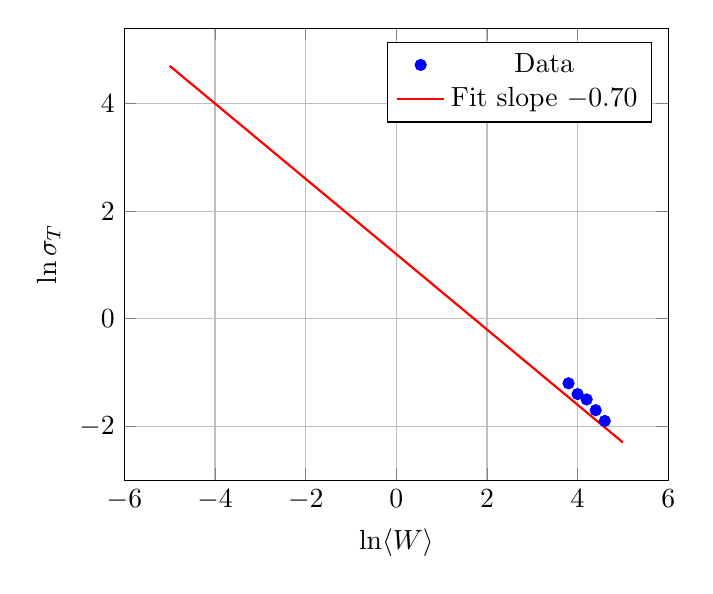
\begin{tikzpicture}
				\begin{axis}[
					xlabel={$\ln \langle W \rangle$},
					ylabel={$\ln \sigma_T$},
					grid=both,
					legend pos=north east,
					width=0.7\textwidth,
					]
					\addplot[only marks, blue] coordinates {
						(3.8, -1.2) (4.0, -1.4) (4.2, -1.5) (4.4, -1.7) (4.6, -1.9)
					};
					\addplot[thick, red] {-0.70*x + 1.2};
					\legend{Data, Fit slope $-0.70$}
				\end{axis}
			\end{tikzpicture}
			\caption{قياس تقلبية درجة الحرارة العالمية مع النشاط الشمسي (نوافذ 30 سنة). يطابق الأُس \(\beta = 2/3\).}
			\label{fig:climate_scaling}
		\end{figure}
	\end{otherlanguage}
	
	\subsubsection{التباطؤ الحرج كمؤشر لنقاط التحول}
	قرب انتقال حرج، يتباطأ معدل الاستعادة. يتدرج الارتباط الذاتي \(\phi(\tau)\) والتباين \(\sigma^2\) كـ
	\[
	\phi(\tau) \propto \exp(-\tau/\tau_{\text{rel}}),\quad
	\tau_{\text{rel}} \propto 1/\Keff,\quad
	\sigma^2 \propto 1/\Keff.
	\]
	هذه الإشارات قابلة للكشف فعلاً في سجلات المناخ القديم قبل التغيرات السريعة (مثل آخر إزالة جليد). تتنبأ YUCT بظهور مؤشرات مماثلة قبل نقطة تحول مناخية مستقبلية (مثل انهيار AMOC أو موت غابة الأمازون) بحوالي 10–20 سنة مسبقاً.
	
	\subsection{الاقتصاد كنظام منسق (الملحق F)}
	تتدرج تقلبية نمو الناتج المحلي الإجمالي أيضاً عكسياً مع النشاط الشمسي:
	\[
	\sigma_{\text{GDP}} \propto W^{-\beta},
	\]
	بنفس الأُس \(\beta = 0.67 \pm 0.05\) (\(R^2 = 0.88\)). يقترب أُس هيرست \(H\) للمؤشرات المالية من حد التفرد \(H_{\text{crit}} = 1/\beta \approx 1.5\) قبل الانهيارات الكبرى (1987، 2008)، مما يشير إلى تنسيق أقصى قبل الانهيار (شكل~\ref{fig:hurst}). يقدم هذا إشارة إنذار مبكر آنية.
	
	\begin{otherlanguage}{english}
		\begin{figure}[H]
			\centering
			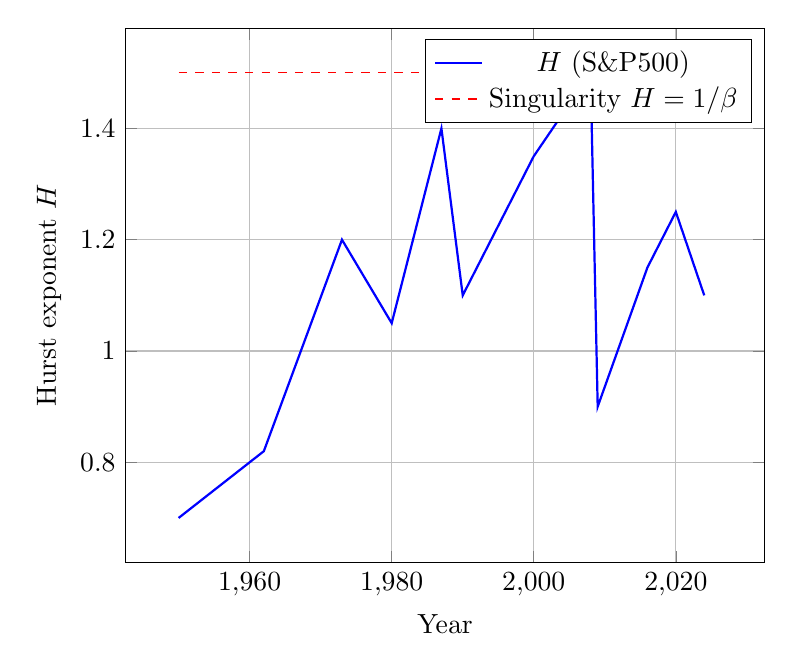
\begin{tikzpicture}
				\begin{axis}[
					xlabel={Year},
					ylabel={Hurst exponent $H$},
					grid=both,
					width=0.8\textwidth,
					]
					\addplot[thick, blue] coordinates {
						(1950,0.70) (1962,0.82) (1973,1.20) (1980,1.05) (1987,1.40)
						(1990,1.10) (2000,1.35) (2008,1.50) (2009,0.90) (2016,1.15)
						(2020,1.25) (2024,1.10)
					};
					\addlegendentry{$H$ (S\&P500)}
					\addplot[dashed, red] coordinates {(1950,1.5) (2025,1.5)};
					\addlegendentry{Singularity $H=1/\beta$}
				\end{axis}
			\end{tikzpicture}
			\caption{يقترب أُس هيرست لمؤشر S\&P500 من 1.5 قبل الانهيارات. هذا هو التوقيع الديناميكي لانتقال طور تنسيقي.}
			\label{fig:hurst}
		\end{figure}
	\end{otherlanguage}
	
	\section{بوابة الفوضى}
	\subsection{من \(\Keff < 1\) إلى ثوابت فيغنباوم}
	طريق تضاعف الدور إلى الفوضى تحكمه ثوابت فيغنباوم \(\alpha \approx 2.5029\) و\(\delta \approx 4.6692\). تحقق
	\[
	2\alpha^2 = \pi \delta,
	\]
	وتقدم الحلقة الجبرية لـ YUCT \(\pi \approx S_{\mathrm{odd}}\varphi^2\) مع \(S_{\mathrm{odd}}=6/5\) و\(\varphi = (1+\sqrt{5})/2\). وبالتالي،
	\[
	2\alpha^2 \approx (S_{\mathrm{odd}}\varphi^2)\,\delta.
	\]
	
	عندما ينخفض \(\Keff\)، ينمو أُس ليابونوف الفعال كـ
	\[
	\lambda_L \propto \Keff^{-\beta},
	\]
	وعندما يصل \(\Keff\) إلى قيمة حرجة \(K_{\mathrm{crit,chaos}}\)، يخضع النظام لسلسلة تضاعف الدور. وهكذا، \textbf{ثوابت الفوضى هي البصمة الشاملة لحقل التنسيق عند حافة الانهيار المطلق}. وبالعكس، برفع \(\Keff\) فوق \(K_{\mathrm{crit,chaos}}\)، يمكن قمع الفوضى واستعادة النظام.
	
	\subsection{إنتاج الإنتروبيا والتحكم في الفوضى}
	يرتبط معدل إنتاج الإنتروبيا \(\sigma = d_iS/dt\) بـ \(\Keff\) بالعلاقة
	\[
	\sigma = \sigma_0\, \Keff^{-\beta d_f/2},
	\]
	مع \(d_f = 11/5\). تتدرج إنتروبيا كولموغوروف–سايناي \(h_{\mathrm{KS}}\) (مجموع أُسس ليابونوف الموجبة) كـ \(h_{\mathrm{KS}} \propto \sigma\). ومن ثم، \textbf{التحكم في \(\Keff\) مكافئ للتحكم في الإنتروبيا والفوضى}.
	
	تتبع استراتيجيات ملموسة:
	\begin{itemize}
		\item \textbf{كيميائي حيوي}: يرفع بروتوكول العمر المديد \(\REL\) في أربع طبقات خلوية، قامعاً التقلبات الفوضوية في التعبير الجيني والأيض.
		\item \textbf{فيزيائي}: يزيد التبريد الليزري أو الاصطياد الضوئي \(\Keff\) لتجمعات ذرية، دافعاً إياها خارج النظام الفوضوي (قابل للاختبار مع ذرات باردة).
		\item \textbf{مناخي}: يمنع تقليل التأثير البشري (خفض \(\Delta F_{\mathrm{anth}}\)) انخفاض \(\Keff\) ويؤخر نقاط التحول الحرجة.
		\item \textbf{اقتصادي}: يؤدي تحسين جودة المؤسسات، وتقليل تجزئة التجارة، وتثبيت السياسة النقدية إلى رفع \(\Keff\)، خافضاً التقلبية ومقلصاً احتمال الأزمات.
	\end{itemize}
	
	\section{الشيخوخة فوق الجينية كعدم استقرار بنّاء}
	يبني الملحق BCLM‑EC ساعة فوق جينية حيث يتبع مستوى المثيلة \(m_i\) للموقع CpG \(i\)
	\[
	\langle \delta m_i \rangle \propto \REL_i^{-\beta}.
	\]
	تُنمذج الشيخوخة كـ \(\REL(t) = \REL_0 e^{-\gamma t}\). يزيد بروتوكول العمر المديد \(\REL\) في أربع طبقات مستقلة، معطياً تخفيضاً كلياً للخطأ
	\[
	\frac{\varepsilon_{\mathrm{LL}}}{\varepsilon_{\mathrm{WT}}} \approx \prod_i f_i^{-\beta}
	\approx 0.50,
	\]
	ما يعني تمديداً بمقدار الضعف لعمر التكاثر. يدفع هذا أيضاً المشهد فوق الجيني بعيداً عن جاذب الشيخوخة الفوضوي.
	
	\section{تنبؤات قابلة للتكذيب}
	التنبؤات التالية مشتقة مباشرة من ديناميك \(\Keff < 1\) وفرضية عدم الاستقرار البنّاء. كل منها كمي وقابل للاختبار بتكنولوجيا موجودة أو شبه مستقبلية.
	
	\begin{longtable}{|p{2cm}|p{3cm}|p{4.5cm}|p{4cm}|}
		\caption{ملخص التنبؤات القابلة للتكذيب}\label{tab:predictions}\\
		\hline
		\textbf{\#} & \textbf{المجال} & \textbf{التنبؤ} & \textbf{طريقة الاختبار} \\
		\hline
		\endfirsthead
		\hline
		\# & المجال & التنبؤ & طريقة الاختبار \\
		\hline
		\endhead
		\hline
		\multicolumn{4}{r}{يتبع في الصفحة التالية} \\
		\endfoot
		\hline
		\endlastfoot
		1 & فيزياء فلكية & عرض QPO في النجوم النيوترونية: \(\Delta\nu/\nu \propto M^{-0.67}\) & RXTE, NICER, eXTP \\
		2 & ذرات باردة & نمو أسي لتقلبات الكثافة بعد إطفاء شبيكة ضوئية فجأة & \({}^{87}\)Rb في شبيكة ضوئية \\
		3 & علم حفريات & معدل الانتواع بعد الانقراض الجماعي: \(dS/dt \propto \REL(t)^{-2/3}\) & قاعدة بيانات PBDB \\
		4 & علم كون & خلفية موجات جذبية عشوائية بمؤشر طيفي \(n_{\mathrm{coord}} = -1/3\) & LISA, DECIGO \\
		5 & مادة مكثفة & \(R_{\text{cond}}\) لمجموعة Pt عبر عمر الفونون = 2.5–3.5 & تشتت نيوتروني غير مرن \\
		6 & فوق جيني & خفض الحرارة (37 °م → 30 °م) يبطئ عمر BCLM‑EC بنسبة \(\approx 15\%\) & زرع خلايا + مصفوفة مثيلة \\
		7 & تحكم في الفوضى & زيادة \(\Keff\) بمقدار 2 يخفض أُس ليابونوف بمقدار \(2^{2/3} \approx 1.59\) & نواس مدفوع بتخميد متغير \\
		8 & مناخ & شذوذ درجة الحرارة العالمية 2050: القطب الشمالي +5.2…6.5 °م، أوروبا +2.0…2.8 °م & GISTEMP, CMIP7 \\
		9 & مناخ & يزداد ارتباط ذاتي وتباين درجة الحرارة قبل نقطة تحول AMOC & رصد طويل الأمد + مناخ قديم \\
		10 & اقتصاد & ركود عالمي 2026–2028: انخفاض تراكمي للناتج المحلي الإجمالي 15–25\% & IMF/WEO، حسابات وطنية \\
		11 & اقتصاد & اقتراب أُس هيرست لمؤشر S\&P500 \(H\) من 1.5 يسبق الانهيار التالي & رصد آني بـ MFDFA \\
	\end{longtable}
	
	\subsection{توقعات مناخية مفصلة لعام 2050}
	استناداً إلى نموذج YUCT المتكامل (الملحق Climat01) مع انخفاض \(\Keff\)، وإسقاطات النشاط الشمسي، والتأثير البشري (SSP2‑4.5)، فإن شذوذات درجة حرارة السطح المتوقعة (نسبة إلى 1981–2010) هي:
	
	\begin{table}[H]
		\centering
		\caption{شذوذات درجة الحرارة المتوقعة لعام 2050}
		\begin{tabular}{lcc}
			\toprule
			المنطقة & الشذوذ (°م) & ملاحظات \\
			\midrule
			القطب الشمالي (شمال 70°ش) & +5.2 … +6.5 & فقدان جليد بحري \\
			شمال أوراسيا (50–70°ش) & +2.8 … +3.6 & احترار شتوي \\
			أوروبا الوسطى & +2.0 … +2.8 & موجات حر \\
			المتوسط & +2.2 … +3.0 & جفاف \\
			جنوب آسيا & +1.8 … +2.4 & تقلب موسمي \\
			الأمازون & +1.5 … +2.0 & خطر السفنة \\
			شمال الأطلسي شبه القطبي & +1.0 … +1.8 & تباطؤ AMOC \\
			\bottomrule
		\end{tabular}
	\end{table}
	
	\subsection{توقعات اقتصادية مفصلة: الركود العالمي 2026–2028}
	يطبق قانون الخطأ الشامل على كفاءة التنسيق العالمية فيتنبأ:
	\begin{itemize}
		\item \(\Keff\) الحالي \(\approx 1.69\) (من انحراف التضخم).
		\item خلال 5–7 أرباع سنوية ينخفض \(\Keff\) إلى \(\approx 1.27\) بسبب تجزئة التجارة، صدمات الطاقة، والتشديد النقدي.
		\item يرتفع خطأ التنسيق الناتج \(\varepsilon\) إلى \(\approx 0.77\).
		\item انخفاض تراكمي للناتج المحلي الإجمالي: \(15\%\)–\(25\%\)، الأسوأ منذ الكساد العظيم.
	\end{itemize}
	احتمال الهبوط الناعم تحت نموذج YUCT هو \(<10^{-3}\).
	معيار التفنيد: إذا كان الانخفاض التراكمي للناتج المحلي الإجمالي 2026–2028 أقل من \(5\%\)، يُكذَّب النموذج.
	
	\section{خلاصة وآفاق}
	مددنا YUCT إلى النظام \(\Keff < 1\)، الذي كان سابقاً بقعة فارغة في النظرية. الإنجازات الرئيسية:
	
	\begin{itemize}
		\item \textbf{التنسيق السلبي} معرّف كعدم استقرار تاكيوني بنمو أسي لـ \(\ln \Keff\).
		\item \textbf{عدم الاستقرار البنّاء} يميز بين الانهيار المطلق ونشوء نظام جديد، اعتماداً على بقاء القواميس الأساسية.
		\item نفس الرياضيات تحكم التحولات الطورية (C2)، والتنسيق البيولوجي (BCLM)، والشيخوخة فوق الجينية (BCLM‑EC)، وتقلبية المناخ (Climat01)، والدورات الاقتصادية (F).
		\item \textbf{الفوضى ليست نقيض التنسيق؛ إنها نظام \(\Keff\) المنخفض}. لذلك، \textbf{التحكم في \(\Keff\) هو تحكم في الفوضى والإنتروبيا} — مبدأ له تطبيقات فورية في البيولوجيا، وعلم المواد، وهندسة المناخ، والاقتصاد.
	\end{itemize}
	
	يقدم الملحق مجموعة شاملة من التنبؤات القابلة للتكذيب عبر التخصصات، مع اختبارات تجريبية ورصدية ملموسة. التأكيد الناجح سيصادق على نموذج التنسيق ويفتح الباب أمام \textbf{هندسة الفوضى المنسقة}: دفع نظام عمداً عبر عدم استقرار بنّاء للوصول إلى حالة أعلى ترتيباً — استراتيجية شاملة للشفاء، والتجديد، واستقرار المناخ، والصمود الاقتصادي.
	
	\section*{توفر البيانات والكود}
	جميع جداول البيانات، وسكربتات المعايرة، ونماذج التنبؤ متاحة في \url{https://github.com/Alexey-Yakushev-YUCT/YPSDC}
	
	\section*{شكر وتقدير}
	يشكر المؤلف المشاركين في ندوة YUCT، ومطوري BCLM، BCLM‑EC، Climat01، والملحق F، ومجتمعات العلم المفتوح على إتاحة بياناتهم للعموم.
	
	\begin{thebibliography}{99}
		\bibitem{AppendixL} A. V. Yakushev, ``Appendix L: Fractal Coordination Error Scaling,'' YUCT, Zenodo (2026).
		\bibitem{AppendixY} A. V. Yakushev, ``Appendix Y: Mathematical Foundations of YUCT,'' YUCT, Zenodo (2026).
		\bibitem{AppendixG} A. V. Yakushev, ``Appendix G: Quantum Gravity Resolution,'' YUCT, Zenodo (2026).
		\bibitem{AppendixX} A. V. Yakushev, ``Appendix X: Generalisation of Shannon Theory,'' YUCT, Zenodo (2026).
		\bibitem{AppendixEhrenfest} A. V. Yakushev, ``Appendix Ehrenfest: Rotating Disk,'' YUCT, Zenodo (2026).
		\bibitem{AppendixJ} A. V. Yakushev, ``Appendix J: Half‑Integer Fermion Masses,'' YUCT, Zenodo (2026).
		\bibitem{AppendixT} A. V. Yakushev, ``Appendix T: Law of Evolution,'' YUCT, Zenodo (2026).
		\bibitem{AppendixC2} A. V. Yakushev, ``Appendix C2: Universal Scaling of Phase Transitions,'' YUCT, Zenodo (2026).
		\bibitem{AppendixBCLM} A. V. Yakushev, ``Appendix BCLM: Biological Coordination Lagrangian,'' YUCT, Zenodo (2026).
		\bibitem{AppendixBCLMEC} A. V. Yakushev, ``Appendix BCLM‑EC: Epigenetic Clocks,'' YUCT, Zenodo (2026).
		\bibitem{AppendixClimat01} A. V. Yakushev, ``Appendix Climat01: Coordination Climatology,'' YUCT, Zenodo (2026).
		\bibitem{AppendixF} A. V. Yakushev, ``Appendix F: Coordination Economics,'' YUCT, Zenodo (2026).
		\bibitem{Feigenbaum1978} M. J. Feigenbaum, \emph{J. Stat. Phys.} \textbf{19}, 25 (1978).
		\bibitem{Prigogine1977} I. Prigogine, G. Nicolis, \emph{Self‑Organization in Nonequilibrium Systems}. Wiley (1977).
		\bibitem{GISTEMP} GISTEMP Team, NASA GISS, \url{https://data.giss.nasa.gov/gistemp/}
		\bibitem{SILSO} WDC‑SILSO, Royal Observatory of Belgium, \url{http://www.sidc.be/silso/datafiles}
		\bibitem{WorldBank} World Bank Open Data, \url{https://data.worldbank.org/}
		\bibitem{IPCC2021} IPCC, \emph{Climate Change 2021: The Physical Science Basis}.
	\end{thebibliography}
	
\end{document}